\subsection{Методика тестирования}

Верификация выполнена на исходном тестовом наборе \texttt{fuzzy/tests/test\_main.cpp}. Сборка проведена командой \texttt{make test}, которая конфигурирует CMake в режиме Release, собирает статическую и разделяемую библиотеки, компилирует \texttt{fuzzy\_tests} и запускает CTest.

Тесты охватывают следующие свойства:

\begin{enumerate}
\item Для U(0,10) проверяются α-срез [7,10] при α=0.7, значения функции принадлежности внутри и вне носителя, а также центр тяжести 20/3.
\item Для арифметики проверяются границы суммы, разности, произведения и частного, интерполированное значение принадлежности и ошибка деления через величину с носителем [-1,1].
\item Для сравнения проверяются знаки центров тяжести и степени возможности для пересекающихся и удалённых величин.
\item Для генератора проверяется диапазон [0,1), среднее 100000 значений, совпадение последовательностей при одинаковом seed и диапазоны параметров 300 сгенерированных величин.
\item Для отбора проверяется выполнение ограничений ширины и окна для каждого возвращённого индекса.
\item Для кластеризации создаются три группы по 30 интервалов вокруг центров 0, 50 и 100. Проверяется согласованность меток внутри групп, различие меток между группами, автоматическое получение трёх кластеров при δ=10 и одного кластера при δ=1000.
\end{enumerate}

Все тестовые условия проходят без ошибок: исполняемый файл сообщил \texttt{100982/100982 checks passed}, а CTest завершил единственный зарегистрированный тест со статусом \texttt{Passed}. Изменение seed изменяет псевдослучайную последовательность, но не нарушает диапазоны и инварианты алгоритмов.

\subsection{Контрольный замер вычислительной эффективности}

Для оценки порядка времени исполнения дополнительно собрана небольшая программа с \texttt{-O2}, связывающаяся с \texttt{build/libfuzzy.a}. На каждой итерации генерировался набор с seed=42, параметрами lo=0, hi=100, w\_min=5, w\_max=30 и 21 уровнем. Затем измерялись генерация и получение α-срезов при α=0.7, k-means++ для k=3 и пороговый алгоритм при δ=5.

\begin{table}[htbp]
\centering
\caption{Контрольные измерения вычислительной эффективности}
\label{tab:perf}
\begin{tabular}{rrrrr}
\toprule
$n$ & Генерация и срезы, мс & $k$-means++, мс & Итерации & Число кластеров \\
\midrule
50 & 0,014 & 0,005 & 10 & 18 \\
100 & 0,011 & 0,003 & 4 & 18 \\
300 & 0,038 & 0,005 & 3 & 22 \\
1000 & 0,119 & 0,071 & 19 & 22 \\
5000 & 1,098 & 0,520 & 28 & 26 \\
\bottomrule
\end{tabular}
\end{table}

Измерения характеризуют один запуск на локальной машине и предназначены для проверки порядка величин, а не для публикации аппаратно независимого бенчмарка. Небольшой разброс между n=50 и n=100 объясняется дискретностью таймера и стоимостью запуска. Начиная с n=300 наблюдается ожидаемое увеличение времени. Пороговая кластеризация в выбранной конфигурации дороже k-means++ из-за сортировки, последовательных уточняющих проходов и динамического числа кластеров.

При n=5000 k-means++ завершился за 0,520 мс после 28 итераций. Пороговый метод занял 11,793 мс и сформировал 26 кластеров при δ=5. Результаты соответствуют различию алгоритмических контуров и не свидетельствуют о деградации памяти в проверенном диапазоне.

\begin{figure}[htbp]\centering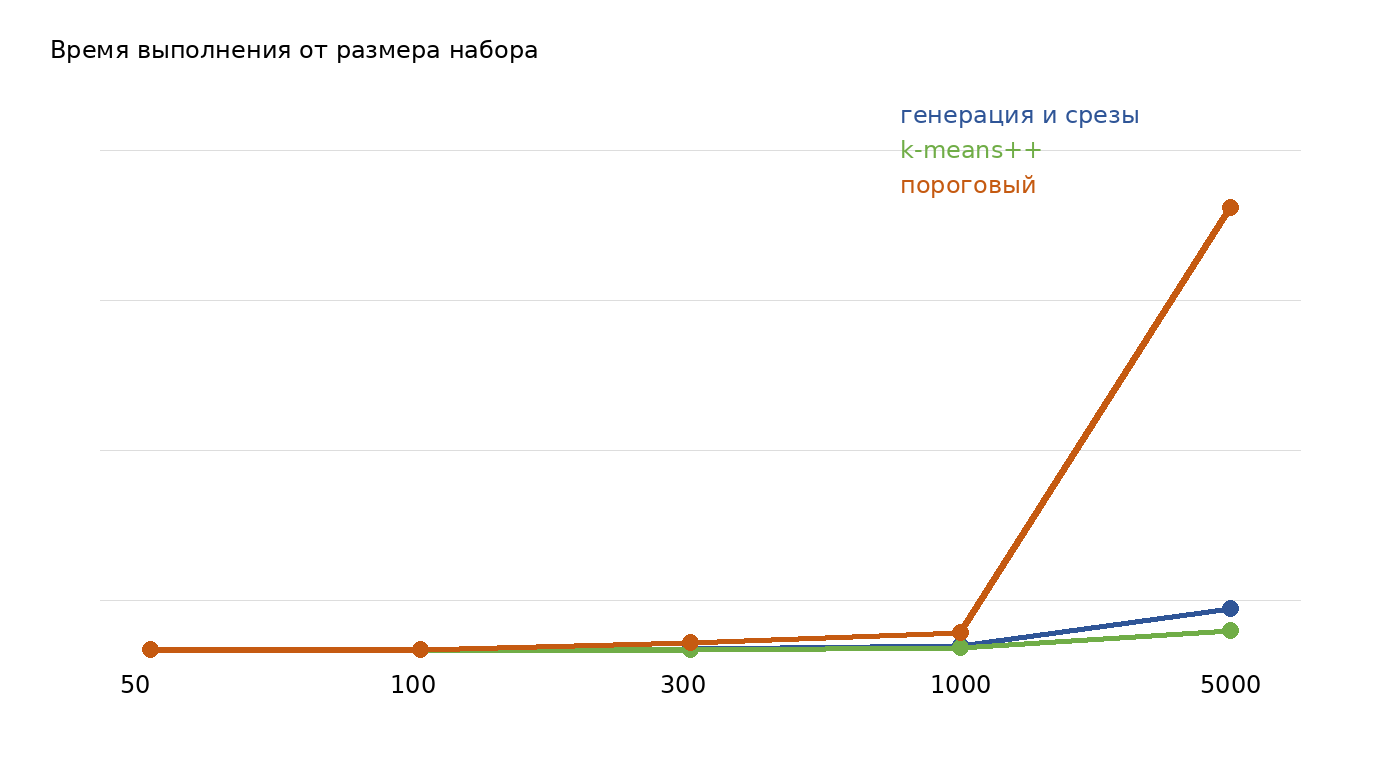
\includegraphics[width=0.9\textwidth]{figures/fig5_time.png}\caption{время выполнения от размера набора}\label{fig:5}\end{figure}

\subsection{Интерпретация результатов кластеризации}

В тесте с тремя синтетическими группами интервалы построены около центров 0, 50 и 100 с малым случайным шумом. k-means++ при k=3 присваивает соседние элементы одной группе одинаковые метки, а три группы получают разные метки. Это показывает, что метрика max(|ΔA|,|ΔB|) согласованно различает разнесённые облака интервалов.

Пороговый алгоритм при δ=10 также выделяет три кластера. Увеличение δ до 1000 приводит к объединению всех объектов в один кластер, поскольку расстояние до единого центра оказывается ниже порога. Тем самым параметр δ управляет компромиссом между компактностью и числом групп. В прикладном запуске δ следует выбирать в масштабе исходной переменной, поскольку он измеряется в тех же единицах, что и A и B.

Для случайного набора из 5000 интервалов при δ=5 число кластеров оказалось равным 26. Это число не является универсальной характеристикой генератора. Оно зависит от seed, диапазона a, диапазона ширин и выбранного α. При увеличении α длина среза уменьшается, что обычно уменьшает вертикальный разброс точек на плоскости (A,B), однако сдвиг A вправо может изменить относительное расположение групп.

\begin{figure}[htbp]\centering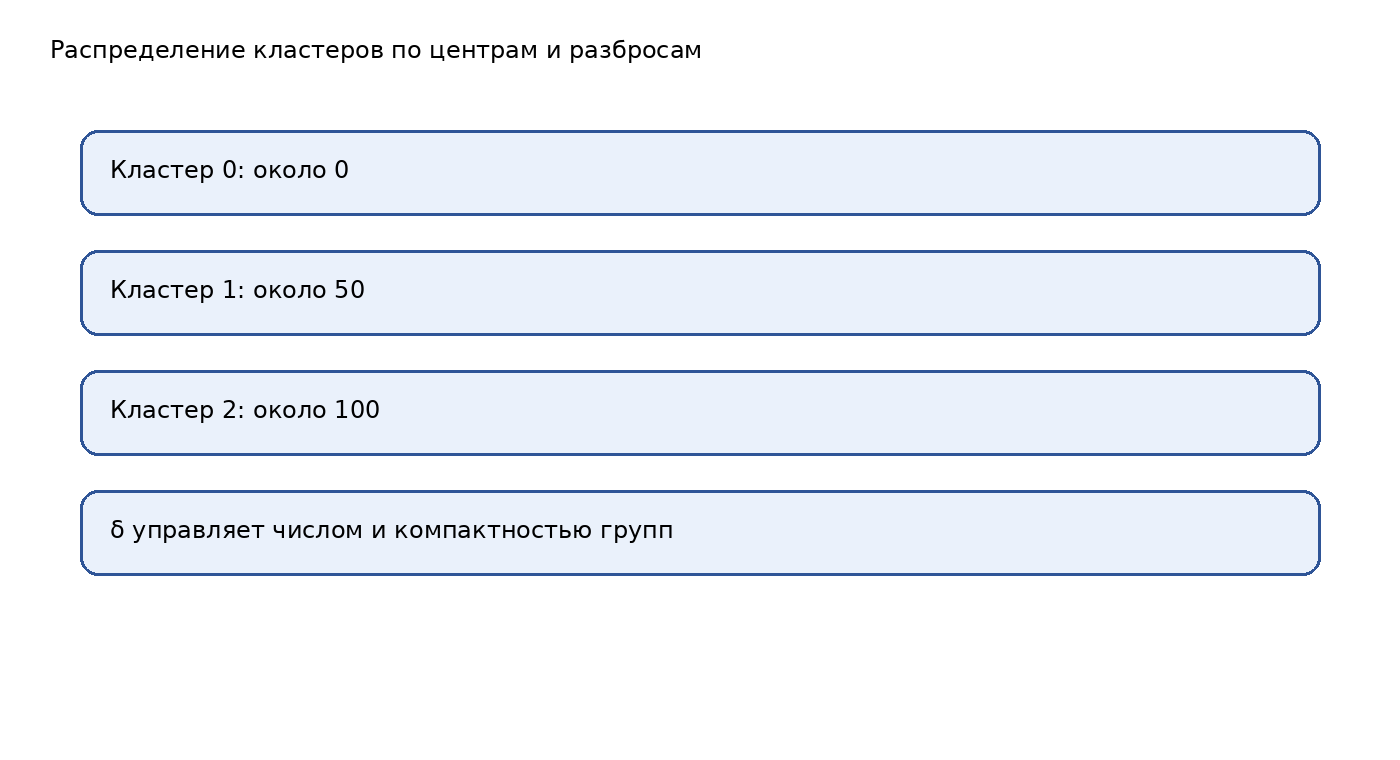
\includegraphics[width=0.9\textwidth]{figures/fig6_clusters.png}\caption{распределение кластеров по центрам и разбросам}\label{fig:6}\end{figure}

\subsection{Проверка корректности интерфейсного контура}

Сервер собирается командой \texttt{make server}, которая сначала собирает библиотеку, затем запускает \texttt{go build -a} с включённым cgo. При обращении к \texttt{/api/generate} параметры запроса проверяются на стороне Go и C++. Снимок состояния содержит исходные a,b, текущий α-срез, признак отбора и метку кластера. После изменения α прежние метки сбрасываются, что исключает рассогласование между данными и визуализацией.

Операционный маршрут \texttt{/api/op} создаёт две величины U(a,b), возвращает исходные срезы, результат операции, центр тяжести, сравнение и два значения Poss. При запрещённом делении результат содержит текст ошибки, полученный из \texttt{fz\_last\_error}, а HTTP-обработчик сохраняет корректный JSON-контракт.

Импорт CSV принимает разделители запятую, точку с запятой, табуляцию и пробел. Экспорт включает столбцы \texttt{id,a,b,A,B,selected,cluster}. Это позволяет использовать результат кластеризации в последующем внешнем анализе.

\subsection{Ограничения экспериментальной части}

Проведённые измерения не заменяют профилирование на целевом оборудовании. В проекте отсутствуют стресс-тесты на многопоточные запросы к серверу, поэтому синхронизация подтверждена анализом кода и сборкой, но не нагрузочным экспериментом. Не исследовалась чувствительность качества кластеров к систематическому изменению α, k и δ по сетке параметров. Эти направления относятся к расширенному исследованию и могут быть включены в выпускную квалификационную работу.

---